%\newcommand{\notatki}{1}
\documentclass{sa}
\usepackage{array} %dla poziomego wyrownania (m) w tabeli
\usepackage{soul}
\usepackage{bm}

\newcommand{\ang}[1]{(ang. \emph{#1})}
\renewcommand{\vec}[1]{\ensuremath\boldsymbol{#1}}
\newcommand{\grad}{\ensuremath\nabla}
\let\avg\overline

\usetikzlibrary{datavisualization}
\usetikzlibrary{datavisualization.formats.functions}

\usepackage{hyperref}
\graphicspath{{06_cnn/}}
\subtitle{Splotowe sieci neuronowe\\Convolutional neural networks}
\begin{document}
\begin{frame}
\titlepage
\end{frame}

\begin{frame}{ImageNet: Large Scale Visual Recognition Challenge}
\begin{block}{Zadanie (jedno z kilku)}
150 tyś. obrazów ręcznie etykietowanych na obecność obiektów z predefiniowanej hierarchii 1000 kategorii.
Celem jest podanie listy 5 kategorii, których obiekty występują na zadanym obrazie.
\end{block}
\pause
\begin{block}{Podsumowanie wyników}
\centering
\begin{tabular}{lr}
rok & błędy \\
\hline
człowiek & $\approx5\%$ \\
\hline
2010 & $28{,}2\%$ \\
2011 & $25{,}8\%$ \\
2012 & $16{,}4\%$ \\
2013 & $11{,}7\%$ \\
2014 & $6{,}7\%$ \\
\pause
2015 & \alert{$3{,}6\%$} \\
2016 & \alert{$3{,}0\%$} \\
2017 & \alert{$2{,}3\%$}
\end{tabular}
\end{block}
\end{frame}

\begin{frame}{Inspiracja biologiczna}
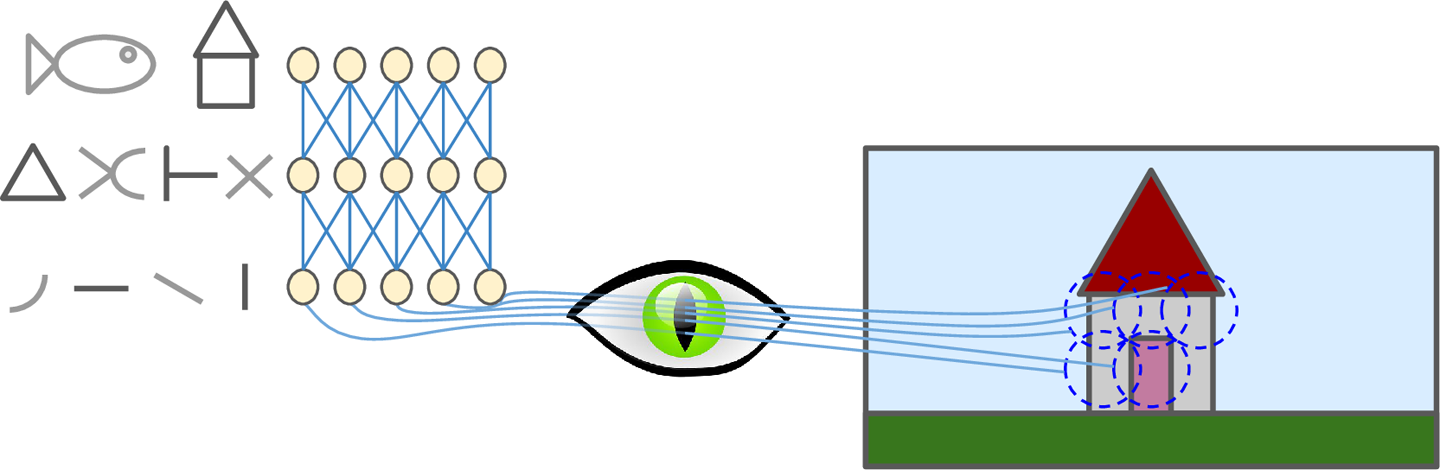
\includegraphics[width=\textwidth]{mlst_1301.png}
{\vfill\footnotesize A. Géron, \emph{Hands-On Machine Learning with Scikit-Learn and TensorFlow} 2017}
\end{frame}

\begin{frame}{Warstwy splotowe}
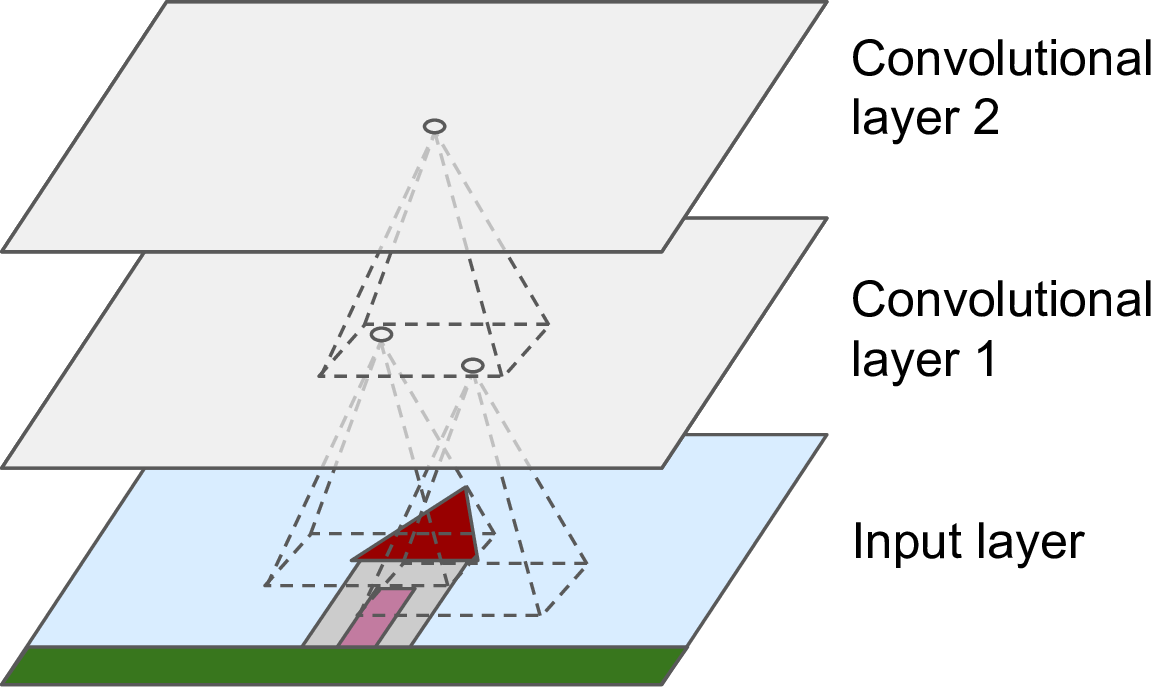
\includegraphics[width=\textwidth]{mlst_1302.png}
{\vfill\footnotesize A. Géron, \emph{Hands-On Machine Learning with Scikit-Learn and TensorFlow} 2017}
\end{frame}

\begin{frame}{Filtr/jądro (ang. \emph{filter/kernel})}
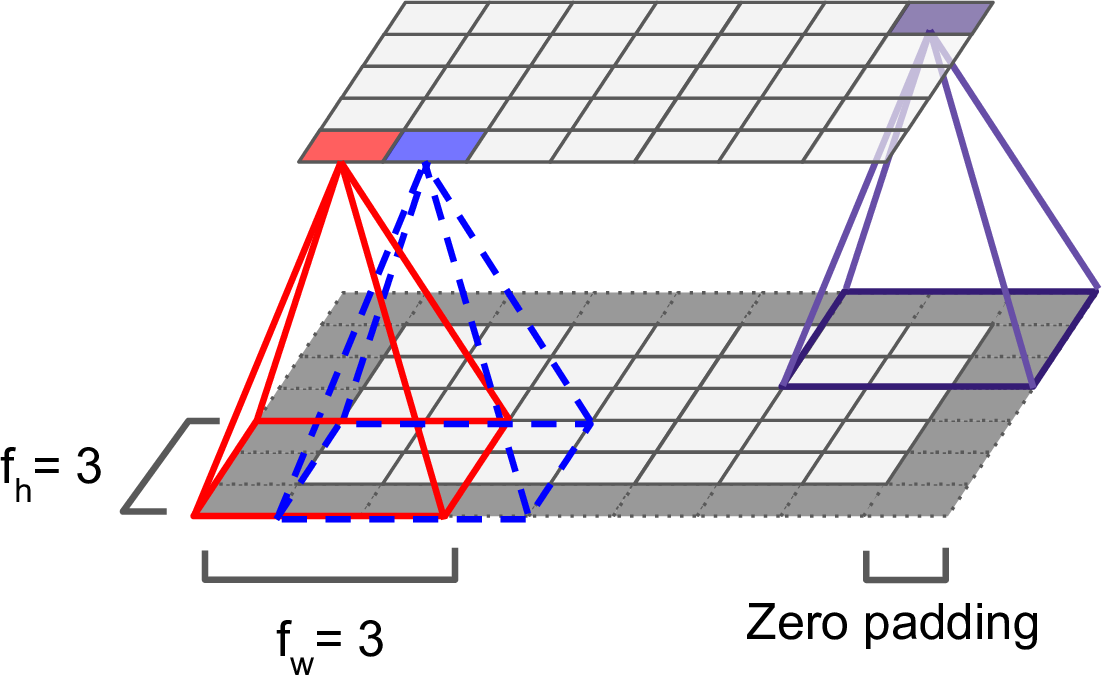
\includegraphics[width=\textwidth]{mlst_1303.png}
{\vfill\footnotesize A. Géron, \emph{Hands-On Machine Learning with Scikit-Learn and TensorFlow} 2017}
\note<1>{Filtr to po prostu suma ważona pikseli pod spodem (+bias), bez nieliniowości}
\end{frame}

\begin{frame}{Krok (ang. stride)}
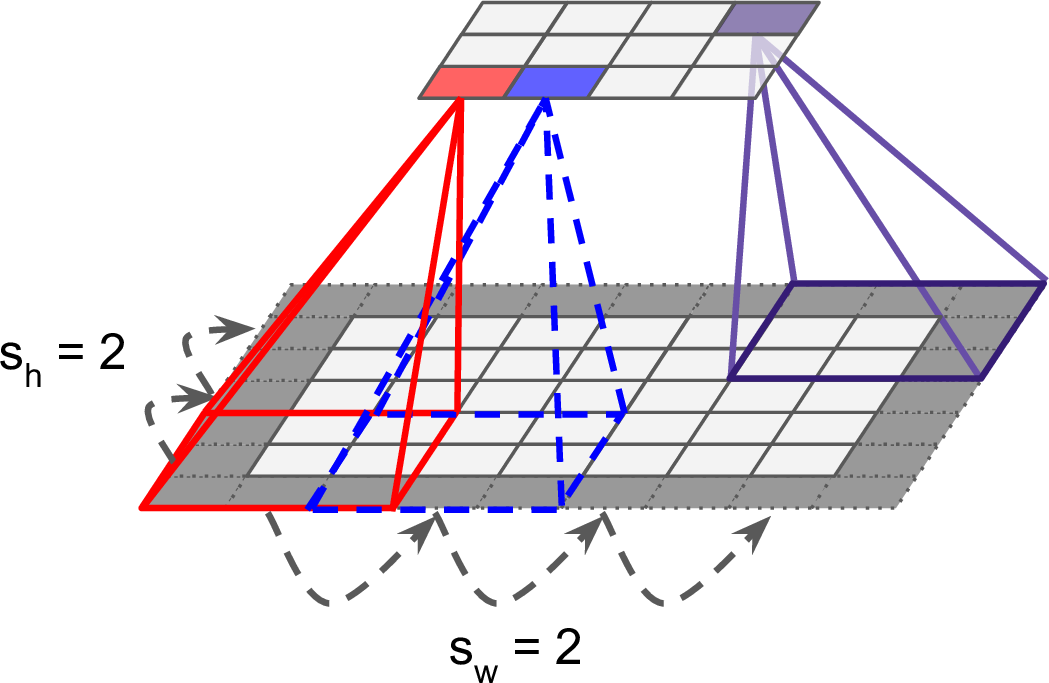
\includegraphics[width=\textwidth]{mlst_1304.png}
{\vfill\footnotesize A. Géron, \emph{Hands-On Machine Learning with Scikit-Learn and TensorFlow} 2017}
\end{frame}

\begin{frame}{Mapa (ang. map)}
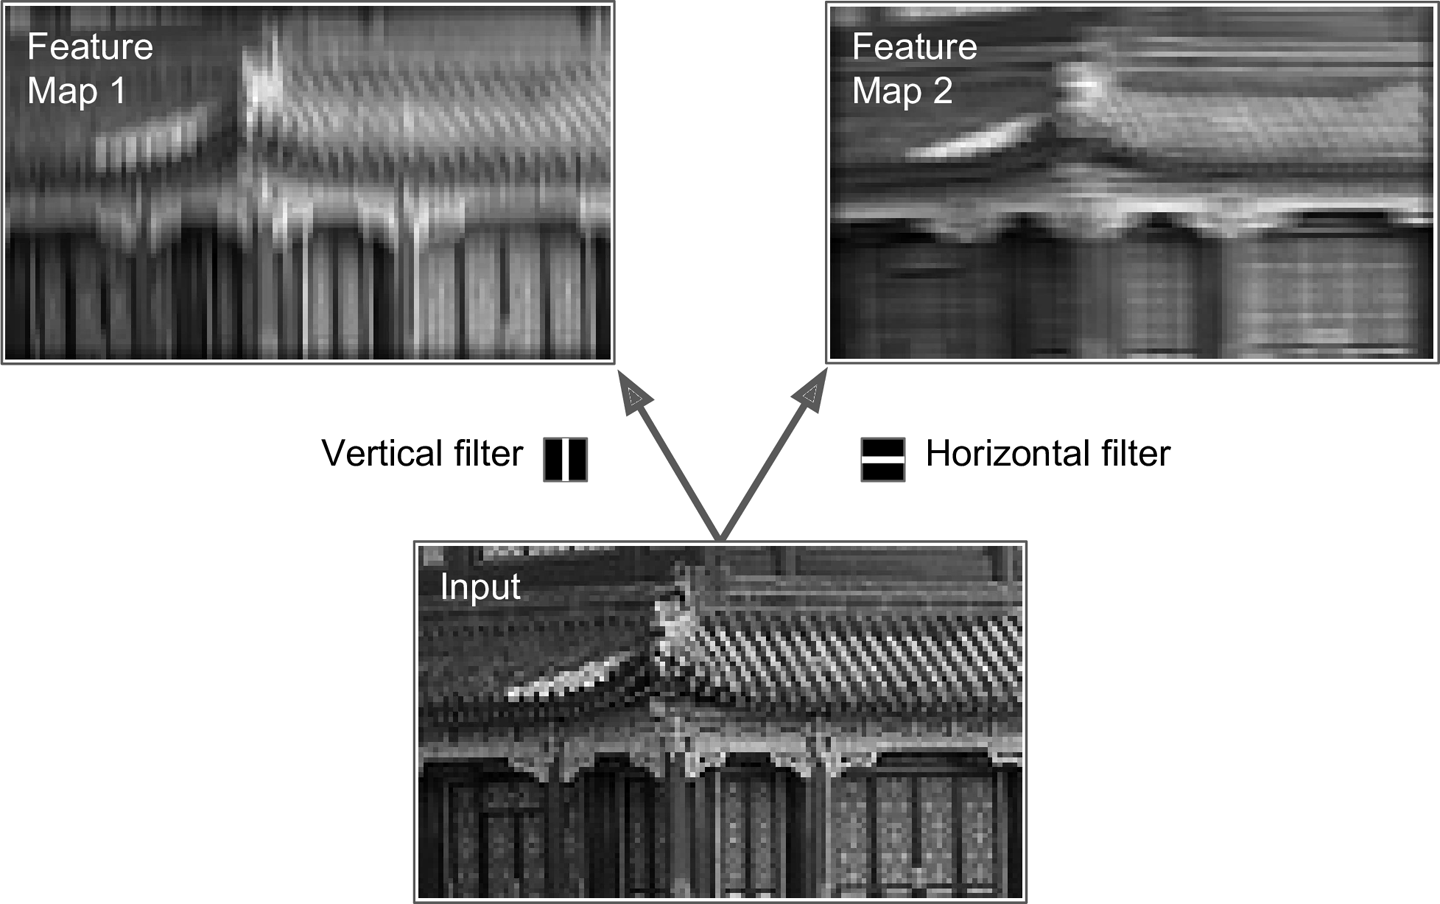
\includegraphics[width=\textwidth]{mlst_1305.png}
{\vfill\footnotesize A. Géron, \emph{Hands-On Machine Learning with Scikit-Learn and TensorFlow} 2017}
\end{frame}

\begin{frame}{Przypadek wielowymiarowy}
\centering
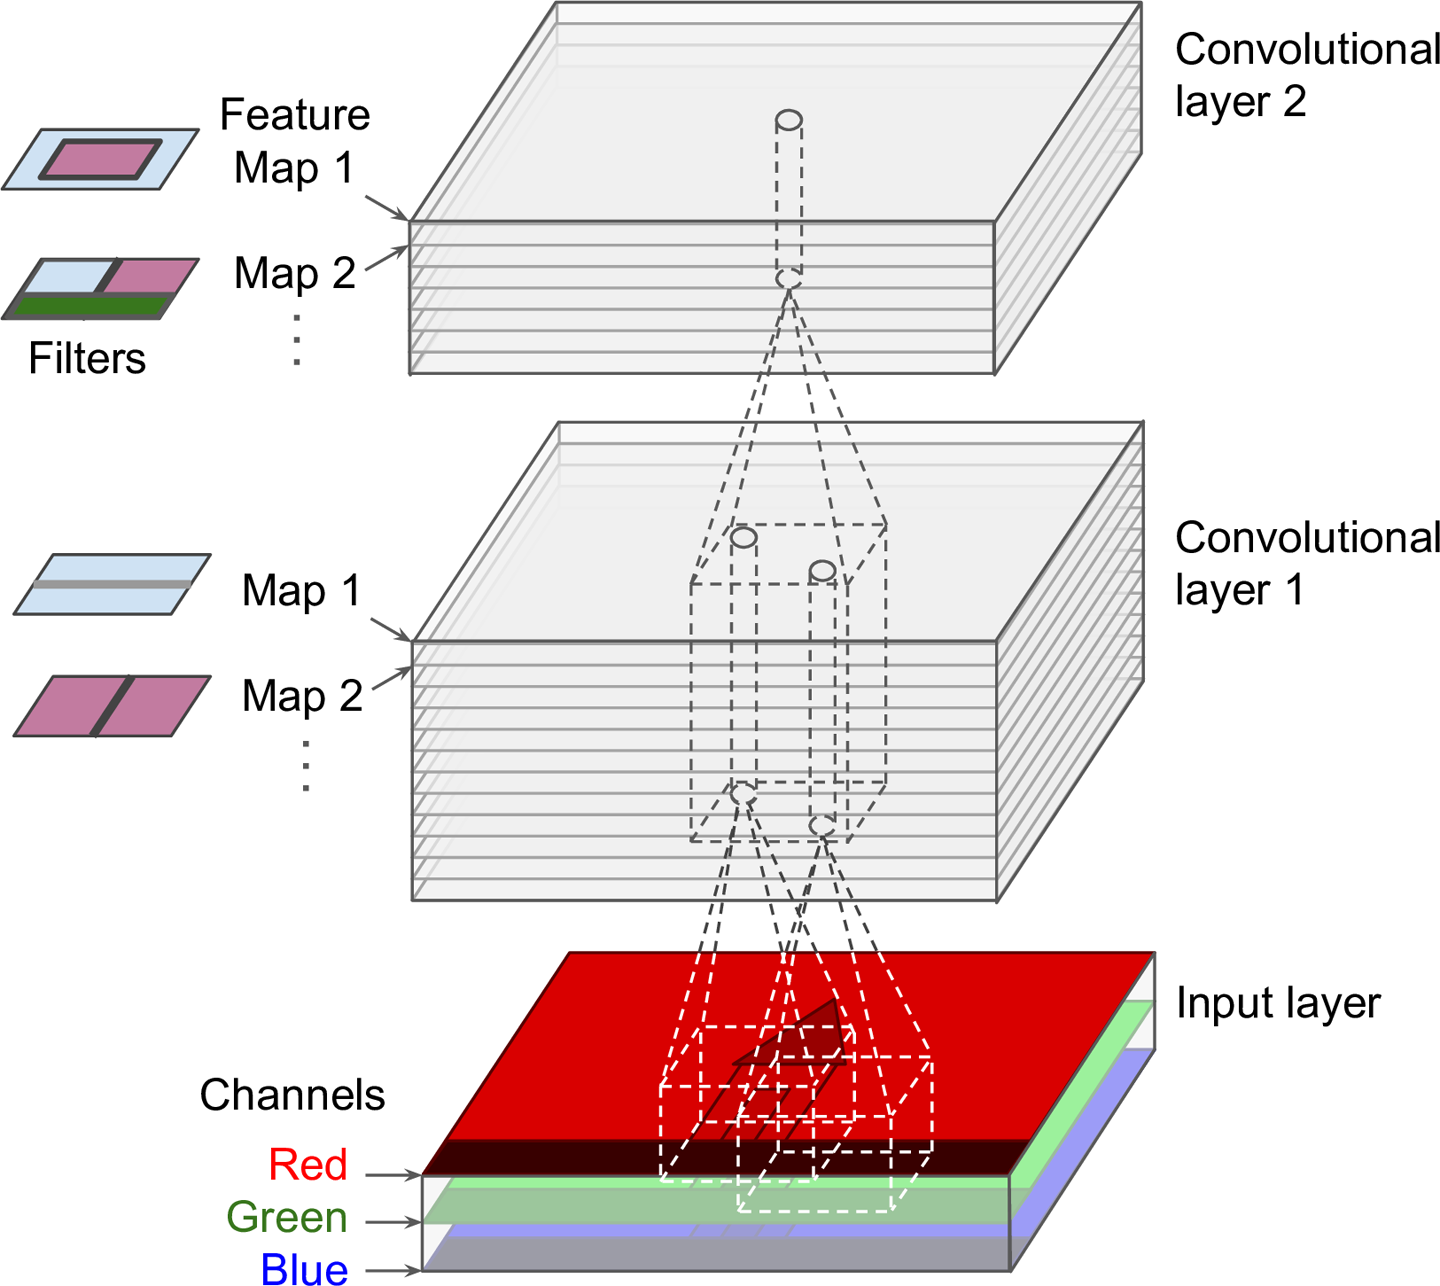
\includegraphics[width=.65\textwidth]{mlst_1306.png}
{\vfill\footnotesize A. Géron, \emph{Hands-On Machine Learning with Scikit-Learn and TensorFlow} 2017}
\end{frame}

\begin{frame}{Padding}
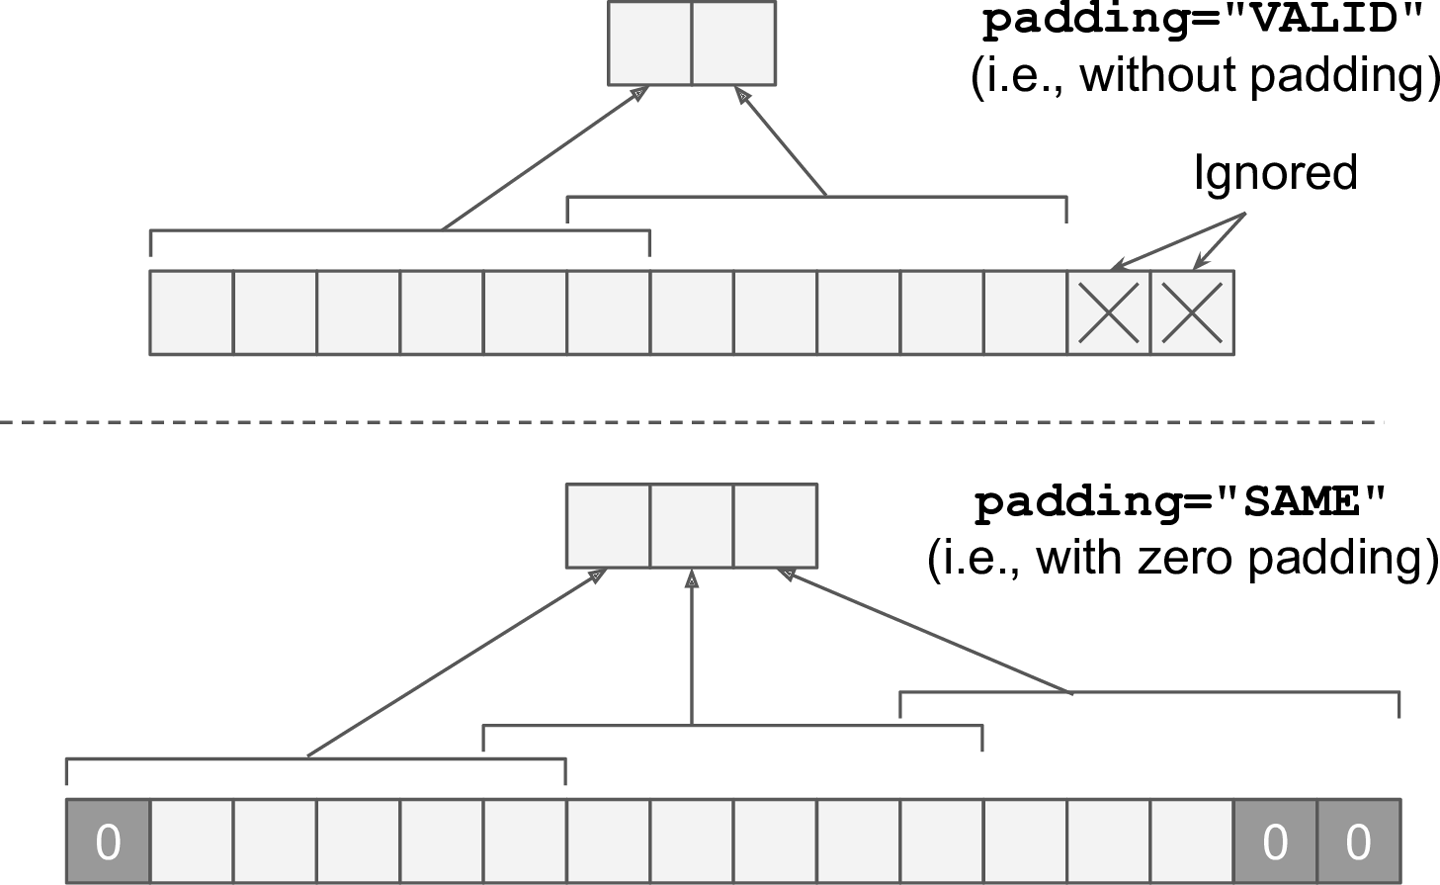
\includegraphics[width=\textwidth]{mlst_1307.png}
{\vfill\footnotesize A. Géron, \emph{Hands-On Machine Learning with Scikit-Learn and TensorFlow} 2017}
\end{frame}

\begin{frame}{Łączenie (ang. pooling)}
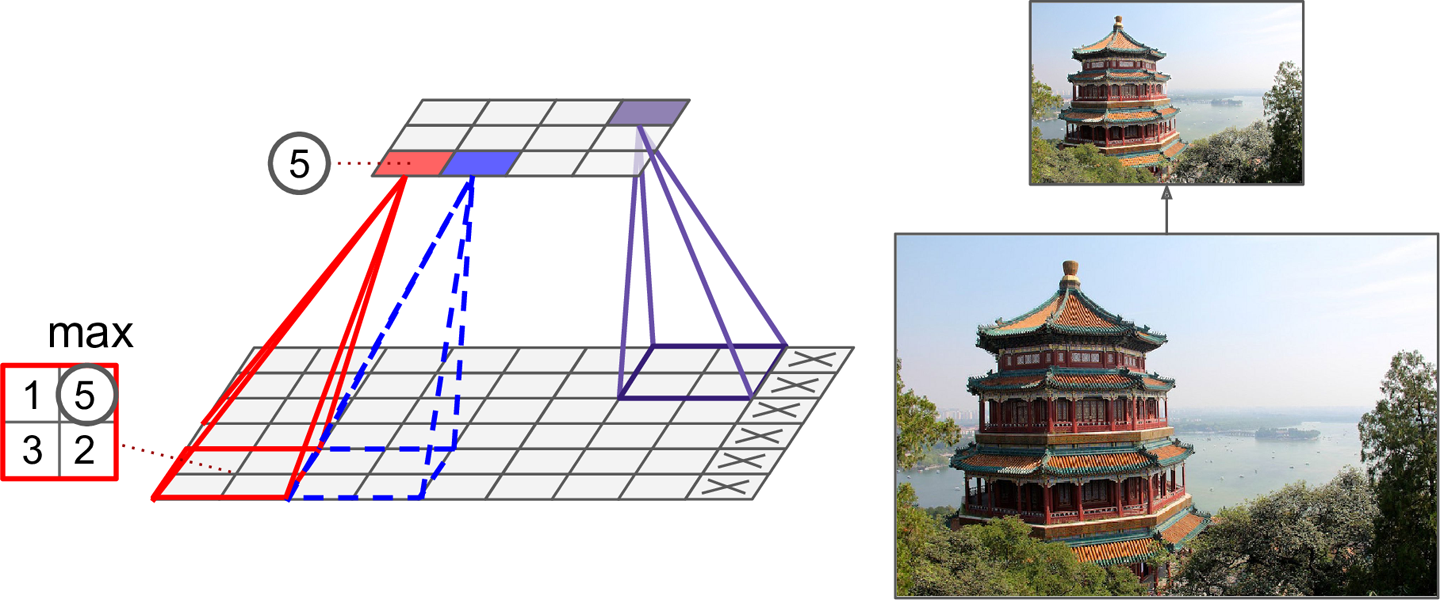
\includegraphics[width=\textwidth]{mlst_1308.png}
{\vfill\footnotesize A. Géron, \emph{Hands-On Machine Learning with Scikit-Learn and TensorFlow} 2017}
\end{frame}

\begin{frame}{Typowa architektura}
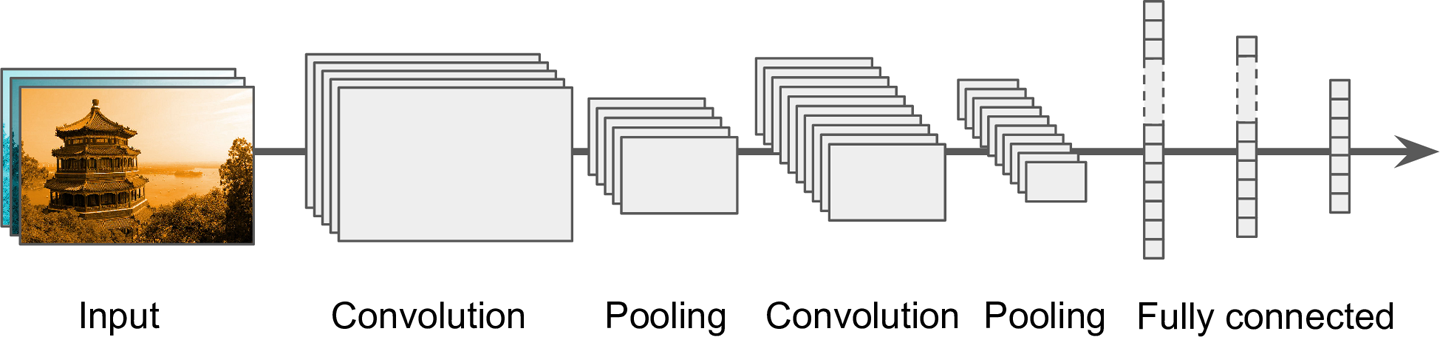
\includegraphics[width=\textwidth]{mlst_1309.png}
{\vfill\footnotesize A. Géron, \emph{Hands-On Machine Learning with Scikit-Learn and TensorFlow} 2017}
\note<1>{Po convolution zwykle jest nieliniowość, np. ReLU}
\end{frame}

\begin{frame}{Przykład: ResNet (ILSVRC 2015)}
\begin{itemize}
\item $3{,}57\%$ w ILSVRC 2015 za pomocą złożenia 6 sieci
\item residual learning
\item bottleneck architecture
\end{itemize}
\end{frame}

\begin{frame}{Residual learning}
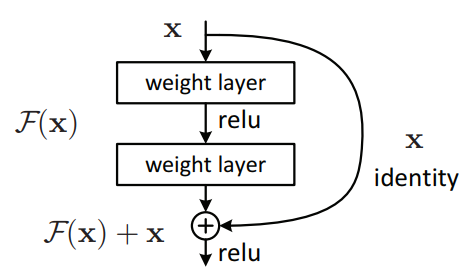
\includegraphics[width=\textwidth]{resnet_fig2.png}
{\vfill\footnotesize K. He et al., \emph{Deep Residual Learning for Image Recognition} \url{https://arxiv.org/pdf/1512.03385v1.pdf}}
\note<1>{$F(x)$ uczy się tylko różnicy pomiędzy $x$ a oczekiwanym wyjściem, co jest łatwiejsze do optymalizacji}
\end{frame}

\begin{frame}{Architektura sieci}
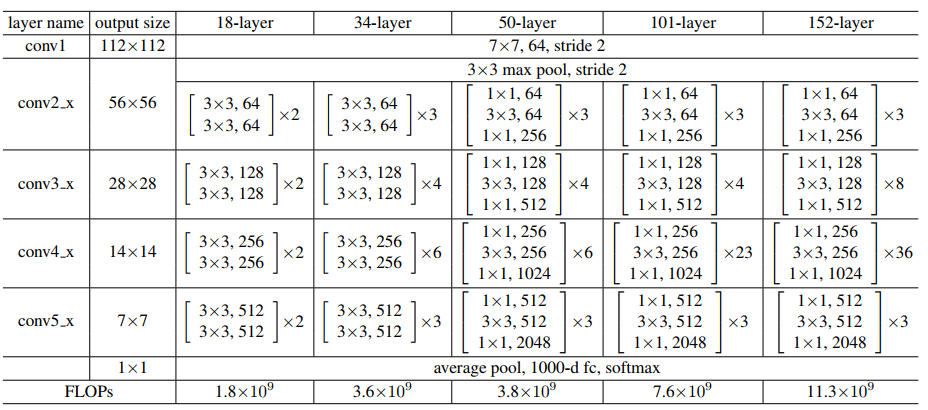
\includegraphics[width=\textwidth]{resnet_tab1.png}
{\vfill\footnotesize K. He et al., \emph{Deep Residual Learning for Image Recognition} \url{https://arxiv.org/pdf/1512.03385v1.pdf}}
\note<1>{Nawiasy kwadratowe oznaczają bloki residual learning (tzn. takie jak pokazano na poprzednim slajdzie). }
\end{frame}

\begin{frame}{Bottleneck architecture}
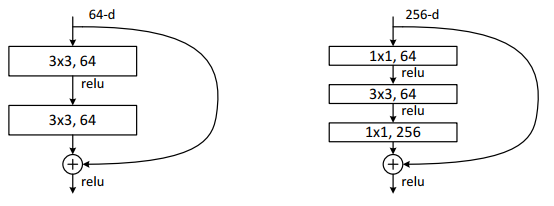
\includegraphics[width=\textwidth]{resnet_fig5.png}
{\vfill\footnotesize K. He et al., \emph{Deep Residual Learning for Image Recognition} \url{https://arxiv.org/pdf/1512.03385v1.pdf}}
\note<1>{Po lewej stronie zwykla architektura, po prawej stronie wariant z bottleneck: pierwsza warstwa zmniejsza liczbe wymiarow, a ostatnia ja odtwarza, dzieki temu srodkowa warstwa (z filtrem $3\times 3$) ma mniejsze wejscie i wyjscie.
Po lewej $3\cdot3\cdot64\cdot64\cdot 2=73728$ parametry, po prawej $64\cdot256+3\cdot3\cdot64\cdot256+256\cdot64=69632$ parametrów: efektywniejsze obliczeniowo, a wydajnościowo podobne.
 }
\end{frame}

\end{document}